\chapter{Projeto de implementação}
\label{cap:projetoimplementacao}

Neste capítulo serão apresentados os serviços considerados críticos para a empresa. Posteriormente, será apresentada uma proposta de solução 
de alta disponibilidade. Essa solução será detalhada na Seção \ref{section:propostasolucao} e será baseada na utilização de virtualização e 
de \textit{softwares} de código aberto. 

\section{Levantamento dos serviços críticos}
\label{section:servcrit}

No capítulo anterior foram detalhados todos os serviços que estão disponíveis na empresa. Nesta seção será feita uma análise desses
serviços, destacando os serviços que foram considerados críticos para a empresa. Para a seleção dos serviços críticos foram adotados os 
seguintes critérios:
\begin{itemize}
 \item A quantidade de clientes que utilizam o serviço: esse é o item mais relevante, pois impacta diretamente no faturamento
 da empresa. De fato, se um cliente ficar sem acesso à Internet, o cliente terá um desconto proporcional ao tempo que ficou sem 
 acesso; 
 \item O número de requisições: esse número é importante, uma vez que, indicam a quantidade de usuários que dependem do serviço e a frequência
 de utilização do serviço. Esse critério engloba, por exemplo, o número de conexões \aca{TCP} \cite{tanenbaum2011}, o número de requisições 
 \aca{UDP} \cite{tanenbaum2011}, a quantidade de acessos em um servidor de hospedagens de sites e a quantidade de requisições \aca{DNS} 
 em um servidor recursivo;
 \item O volume de elementos do serviço: essa medida demonstra a abrangência do serviço, ou seja, quantos clientes são dependentes deste. 
 Como exemplo de elementos pode-se citar a quantidade de contas de \textit{e-mail} ativas em um servidor de \textit{e-mail} ou a quantidade de 
 equipamentos monitorados por um servidor.
 %Esse critério é importante pois com ele pode-se comparar diferentes serviços possibilitando perceber o grau de relevância que cada um possui;
 %Esse critério, como o anterior, também permite comparar diferentes serviços para ter a possibilidade de ordená-los de acordo com sua relevância, por isso o torna importante para esta análise.
\end{itemize}

Nas próximas seções serão descritos os serviços que foram considerados mais críticos, com base nos critérios adotados.

\subsection{DNS recursivo primário}
\label{section:dnsrecprim}

Esse serviço foi classificado como o serviço mais importante pois possui um impacto direto nos clientes do provedor. Além disso, esse é o único 
serviço que todos os clientes e funcionários utilizam, totalizando aproximadamente 9000 pessoas. O objetivo de um provedor é fornecer uma navegação 
de qualidade aos seus clientes, sendo assim, o \ac{DNS} é fundamental para essa navegação. A importância deste serviço está ilustrada na Figura 
\ref{fig:dns_udp} (a), onde pode ser observado que esse serviço possui picos de aproximadamente 1150 requisições por segundo. Já na Figura 
\ref{fig:dns_udp} (b) pode ser observado que o servidor \textit{Passata} é o servidor que apresenta o maior número de requisições 
\ac{UDP}\footnote[1]{Esse número de requisições \ac{UDP} é elevado devido ao fato do serviço \ac{DNS} utilizar esse protocolo de transporte.}. 
Essa figura compara os principais servidores da empresa através de requisições \ac{UDP} e pode ser usada como um indicador da quantidade de 
clientes que utilizam os serviços.

\begin{figure}[h!]
 \centering
 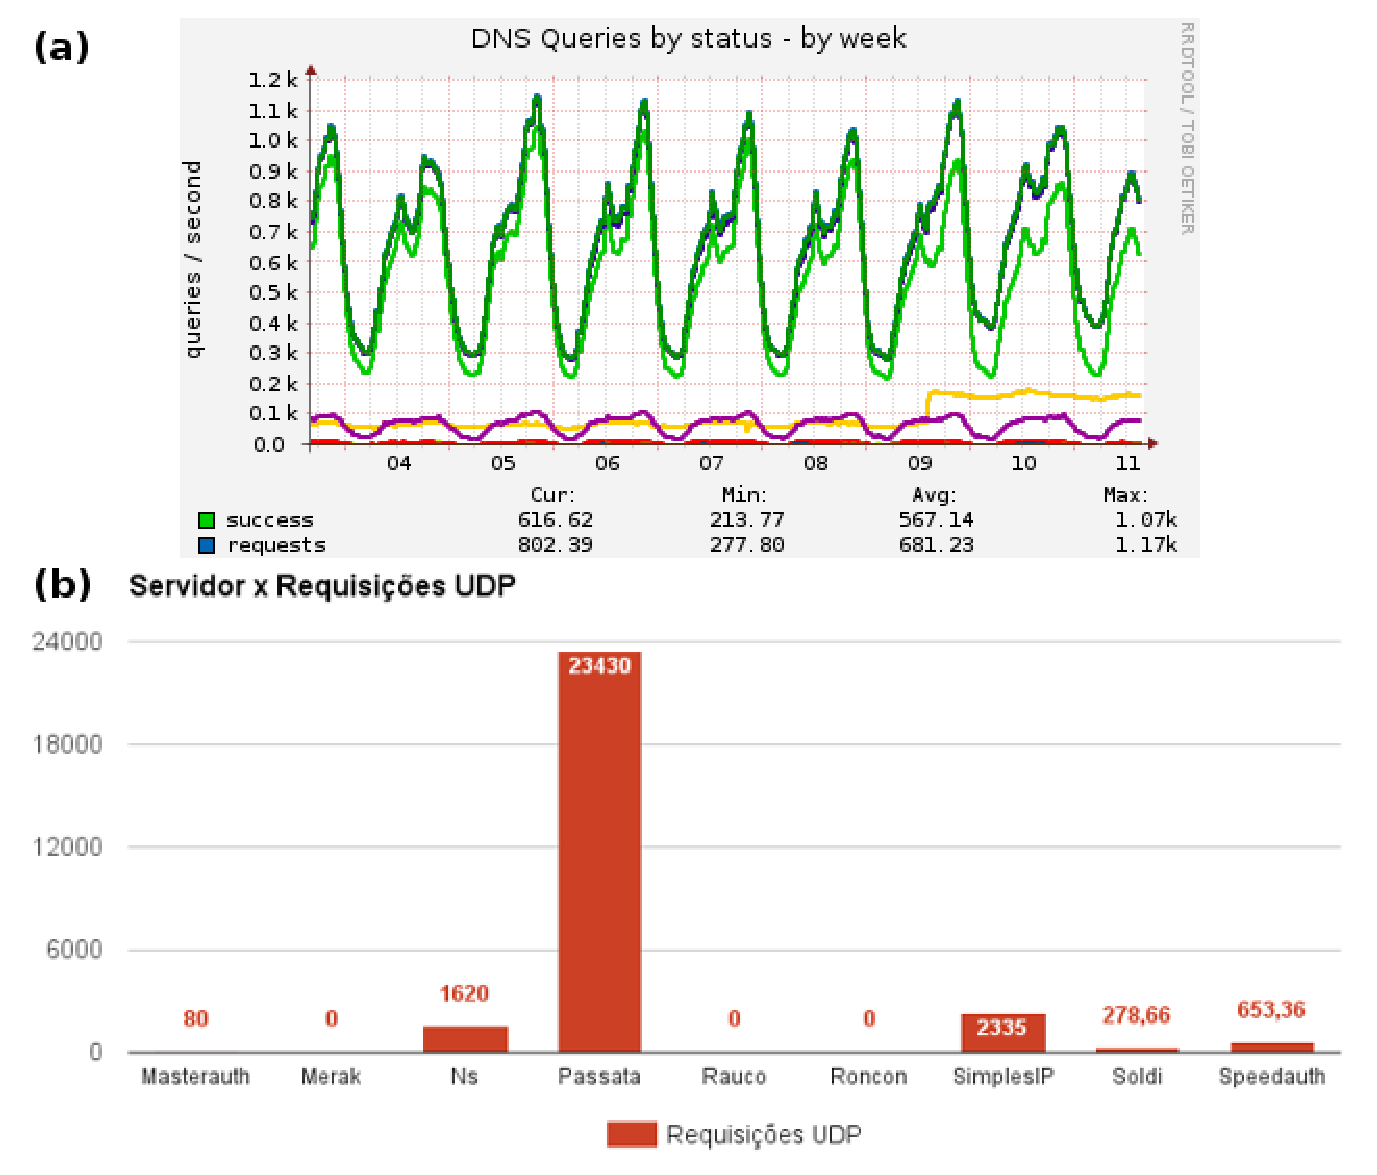
\includegraphics[width=400px]{img/dns_udp.eps}
 \caption{Gráfico de requisições DNS (a) e comparação de requisições UDP entre os principais servidores (b).}
 \label{fig:dns_udp}
\end{figure}

\subsection{Autenticação Radius}
\label{section:radius}

Esse serviço é importante pois é o responsável pela autenticação de todos os clientes do provedor. Caso esse serviço fique indisponível, 
os clientes não conseguirão estabelecer conexão e, consequentemente, não conseguirão utilizar o serviço de Internet. Os servidores 
\textit{Masterauth} e \textit{Speedauth} fornecem o serviço de \textit{Radius}, sendo que recebem em média 1,6 requisições de autenticação 
por segundo. Além disso, esses servidores armazenam dados relacionados à conexão dos clientes, como por exemplo, o endereço de \ac{IP} que é 
utilizado por um cliente em um determinado período de tempo, o tráfego de dados da conexão, o tempo da conexão de cada cliente, o endereço 
\aca{MAC} dos equipamentos dos clientes, entre outros. Essas operações resultam em média 23 requisições por segundo. 
Outro critério que é relevante para esses servidores é o volume de elementos do serviço, que neste caso, representa a quantidade de clientes que
utilizam esses servidores para autenticação. Como pode ser observado na Figura \ref{fig:elementos_tcp} (a), os servidores \textit{Masterauth} e 
\textit{Speedauth} estão entre os que apresentam o maior número de elementos. Além disso, nesses servidores existe um grande número de conexões 
\ac{TCP}\footnote[1]{Esse número de conexões \ac{TCP} deve-se ao fato do \textit{software} \textit{Freeradius} utilizar para comunicação com o
seu banco de dados.}, como pode ser observado na Figura \ref{fig:elementos_tcp} (b).

% \begin{figure}[h!]
%  \centering
%  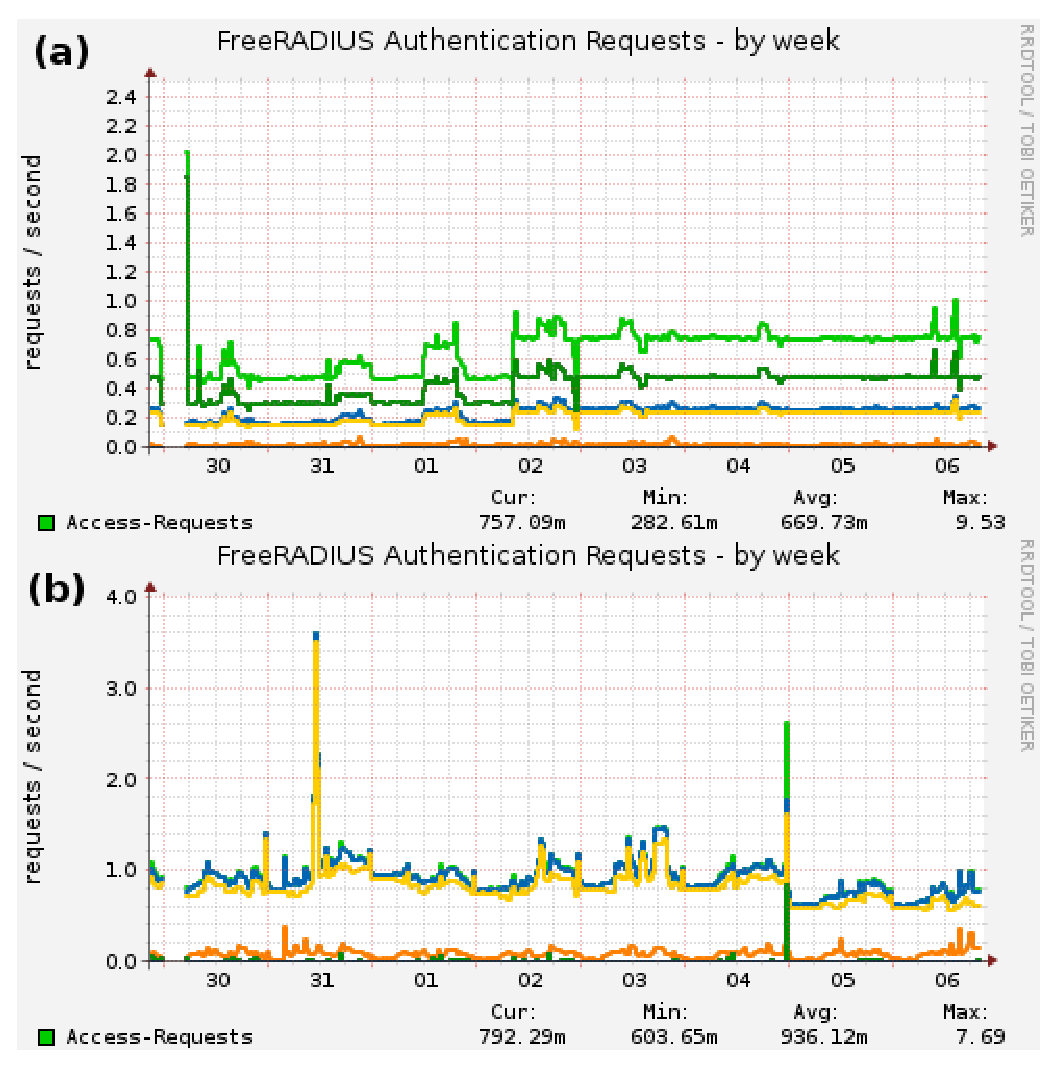
\includegraphics[width=300px]{img/freeradius_auth.eps}
%  \caption{Gráfico de requisições de autenticação do servidor \textit{Masterauth} (a) e \textit{Speedauth} (b).}
%  \label{fig:freeradius_auth}
% \end{figure}

\begin{figure}[h!]
 \centering
 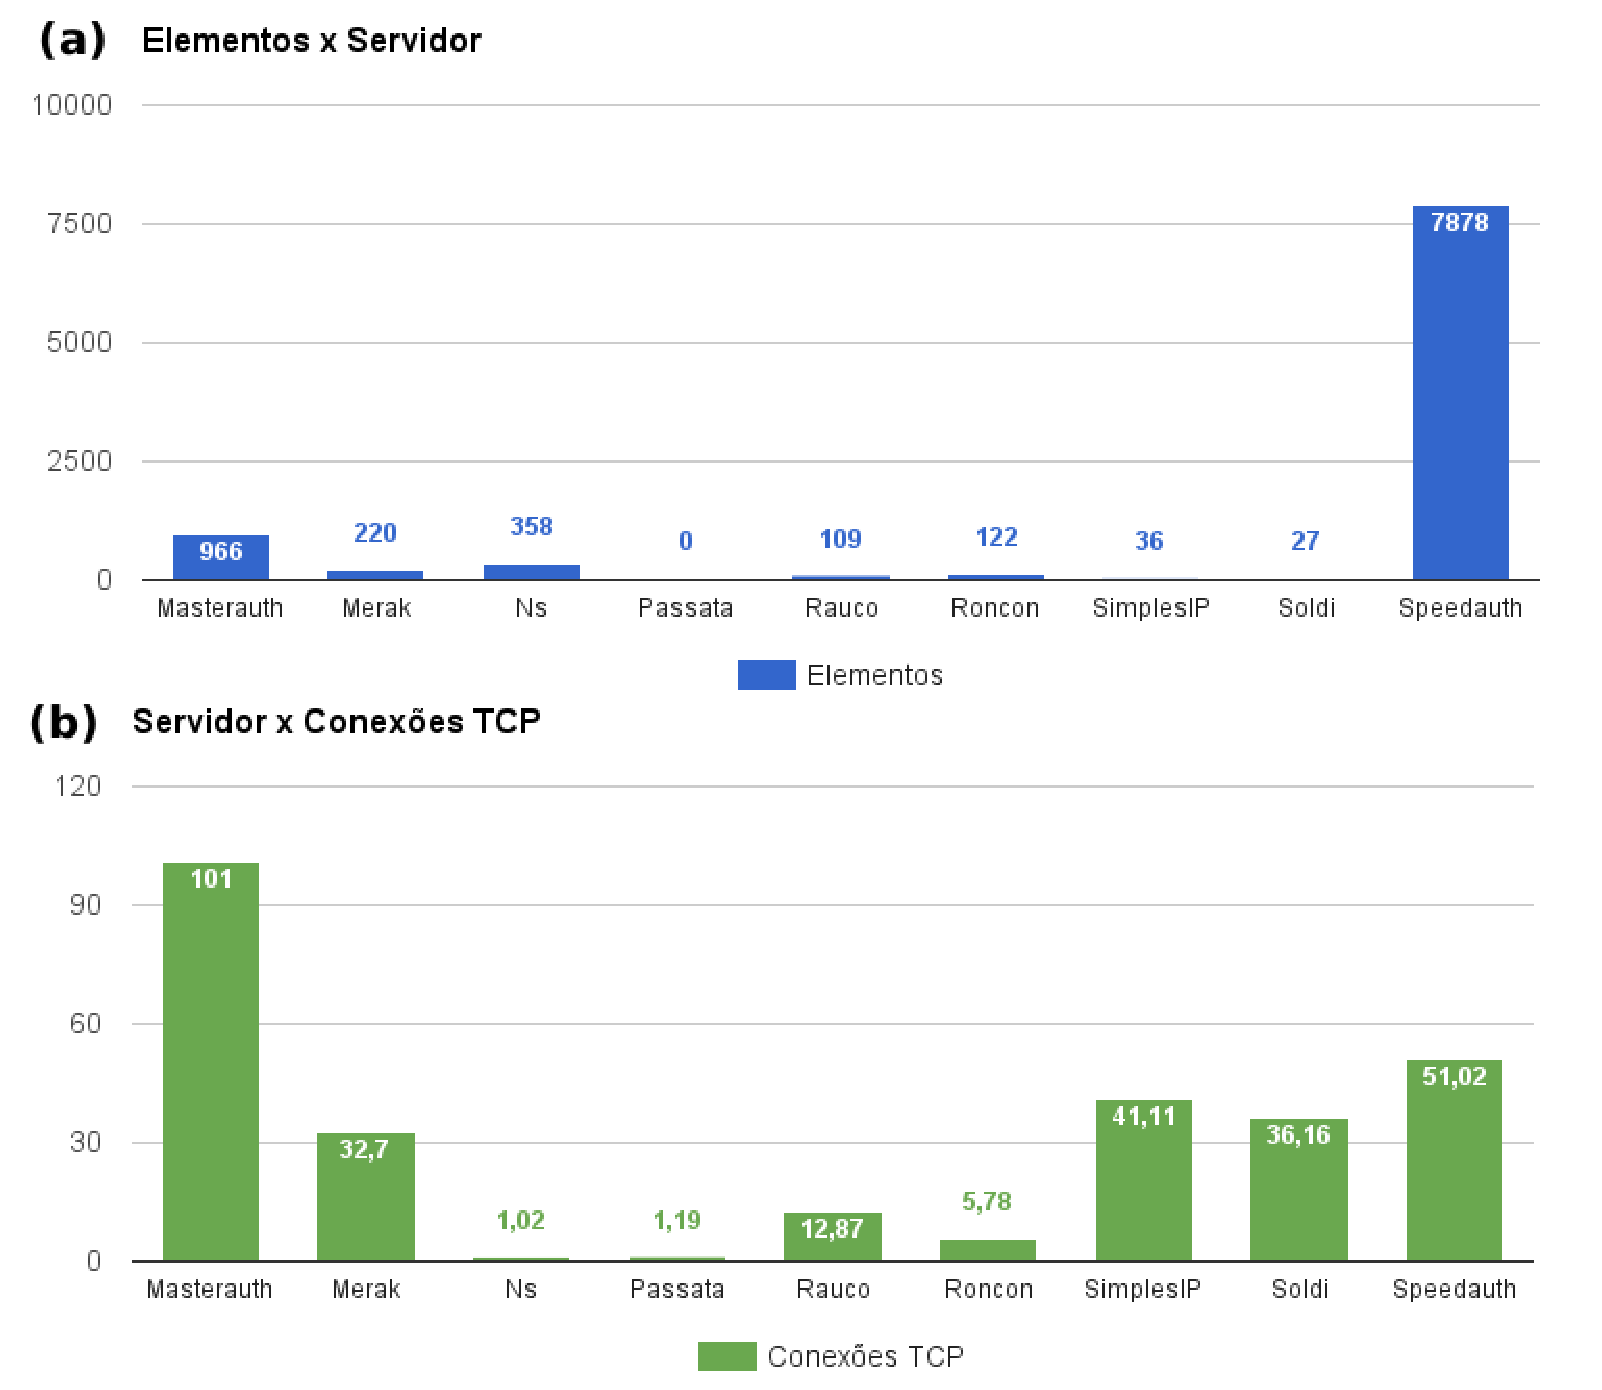
\includegraphics[width=380px]{img/elementos_tcp.eps}
 \caption{Gráfico de comparação de elementos (a) e de conexões TCP (b) entre os principais servidores.}
 \label{fig:elementos_tcp}
\end{figure}

\subsection{Sistemas da empresa e do provedor}
\label{section:sistemas}

O sistema do provedor é responsável pela maior parte das operações gerenciais do provedor. Este sistema é responsável pela emissão de 
boletos, atendimento de clientes, comunicação interna da empresa, vendas, ativações de novos clientes, entre outros. Esse sistema não tem um 
impacto direto para os clientes, porém é fundamental para o funcionamento da empresa e do provedor. Caso haja uma indisponibilidade desses sistemas 
a maior parte dos funcionários ficarão impossibilitados de trabalhar, sendo que a empresa possui um total de 65 funcionários.
%, sendo que são aproximadamente 35 funcionários simultâneos (de acordo com a Figura \ref{fig:ejabberd_week}), isso poderia gerar um prejuízo elevado para a empresa e o provedor. 

O sistema do provedor é executado no servidor \textit{Soldi} que recebe aproximadamente 3 requisições \aca{HTTP} \cite{tanenbaum2011} por segundo
(Figura \ref{fig:soldi_week}). Além disso, a empresa mantém 28 sistemas de outros clientes nesse servidor. 
Como pode ser observado na Figura \ref{fig:elementos_tcp} (b), esse servidor encontra-se entre os que apresentam um alto nível de conexões 
\ac{TCP}\footnote[1]{O número de conexões \ac{TCP} é considerado devido ao fato do protocolo \ac{HTTP} utilizar esse 
protocolo de transporte.}.

%\begin{figure}[h!]
% \centering
% 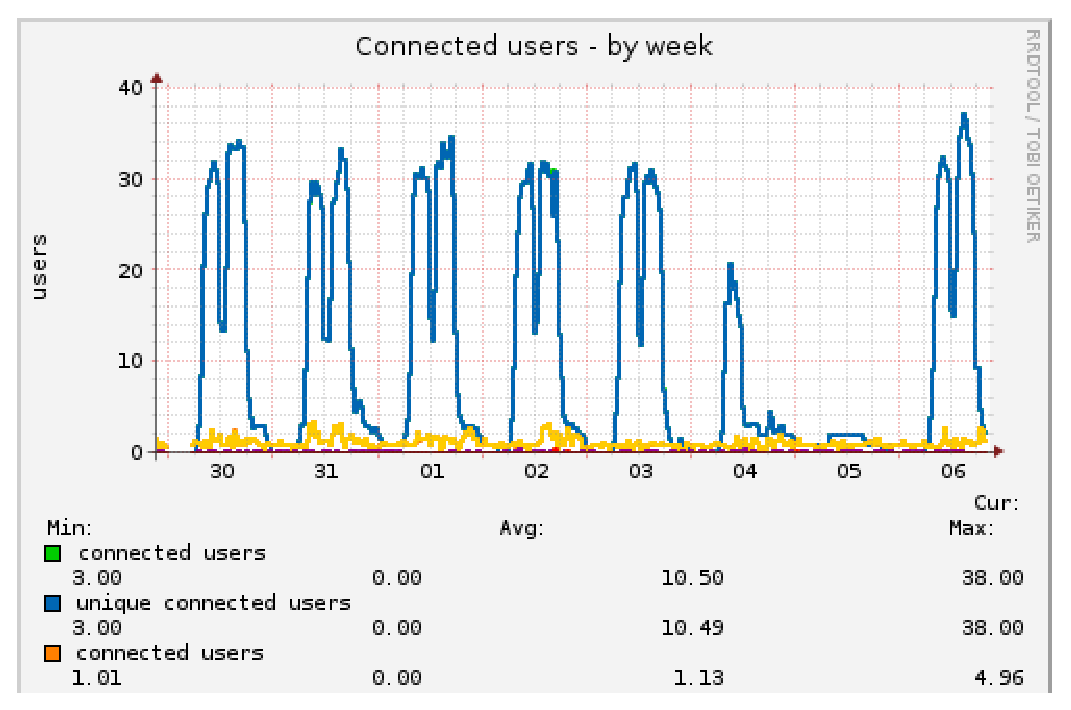
\includegraphics[width=310px]{img/ejabberd_week.eps}
% \caption{Gráfico usuários simultâneos de sistema.}
% \label{fig:ejabberd_week}
%\end{figure}

\begin{figure}[h!]
 \centering
 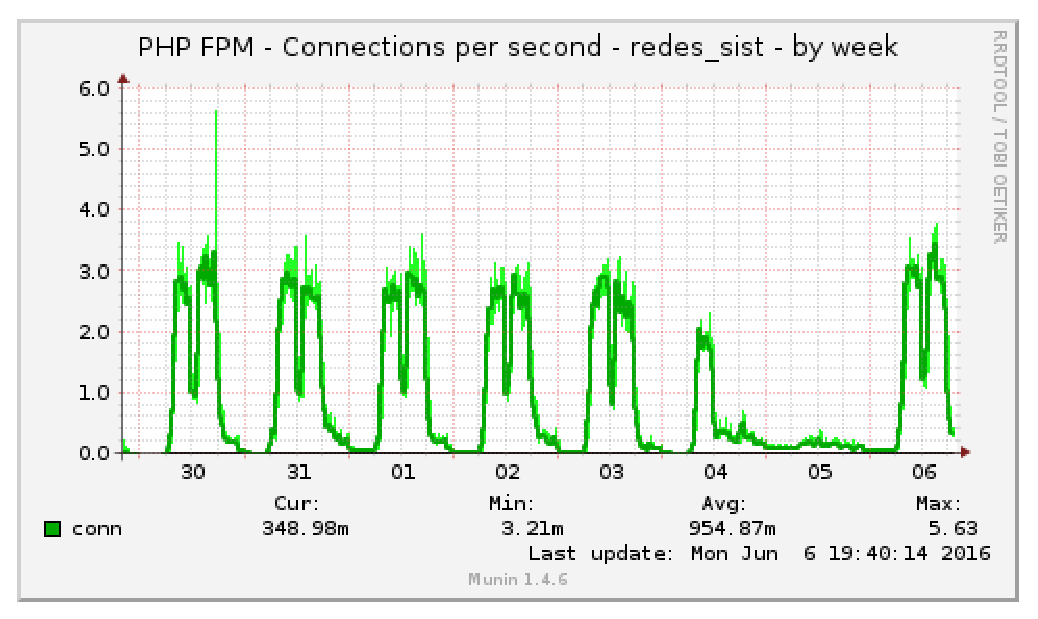
\includegraphics[width=280px]{img/soldi_week.eps}
 \caption{Gráfico de requisições por segundo do maior sistema.}
 \label{fig:soldi_week}
\end{figure}

\subsection{Telefonia interna sobre IP}
\label{section:telefonia}

Esse serviço tem relevância para a empresa e para o provedor, pois permite a comunicação entre os clientes e os funcionários. De fato, o 
servidor \textit{SimplesIP} é responsável por garantir o atendimento dos clientes para fins de suporte técnico, comunicação interna entre 
funcionários, comunicação com técnicos externos, vendas, cobranças a clientes, entre outros. Para quantificar, no mês de maio de 2016 a empresa 
recebeu 15922 ligações, com duração total de 67 horas e 40 minutos. Além disso, no mesmo mês foram efetuadas 674 ligações entre funcionários. 
O gráfico da Figura \ref{fig:simplesip_week} mostra a quantidade de canais ativos no servidor de telefonia. Observa-se que ocorrem 
de 20 a 30 ligações simultâneas durante o horário comercial, que é das 08:00 às 12:00 e das 13:00 às 18:00. Também pode-se observar, na Figura 
\ref{fig:dns_udp} (b), que esse serviço possui um elevado número de requisições \ac{UDP}\footnote[2]{Esse número de requisições \ac{UDP} 
deve-se ao fato da telefonia utilizar o protocolo \ac{UDP} para transmissão de voz.}, se comparado aos demais servidores.

\begin{figure}[h!]
 \centering
 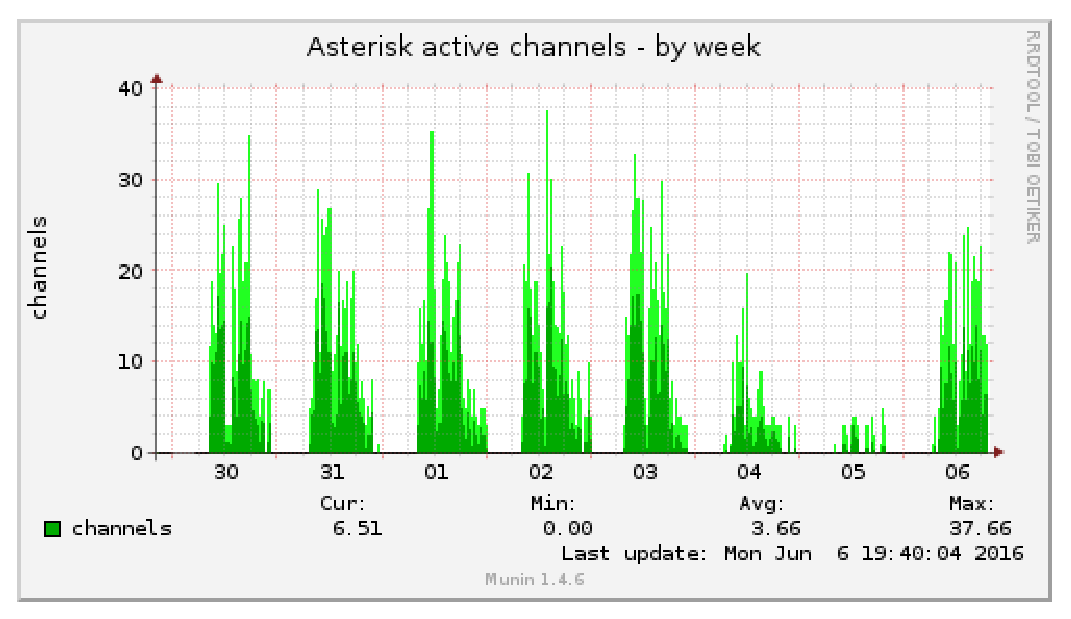
\includegraphics[width=280px]{img/simplesip_week.eps}
 \caption{Gráfico da quantidade de canais ativos no servidor de telefonia.}
 \label{fig:simplesip_week}
\end{figure}

\subsection{Situação atual}
\label{section:maqservcrit}

A partir da análise inicial, verificou-se que os servidores a serem incluídos no ambiente de alta disponibilidade são:
\begin{itemize}
 \item \textit{Passata}: servidor de \ac{DNS} recursivo utilizado tanto pelo provedor quanto pela empresa;
 \item \textit{Speedauth}: servidor \textit{Radius} para autenticação dos clientes do provedor;
 \item \textit{Masterauth}: servidor \textit{Radius} para autenticação dos clientes do provedor;
 \item \textit{Soldi}: servidor dos sistemas gerenciais da empresa e do provedor;
 \item \textit{SimplesIP}: servidor de telefonia sobre \ac{IP} para atendimento dos clientes e comunicação interna do provedor e da empresa;
\end{itemize}

Na Tabela \ref{tab:dispservcrit}, tem-se esses servidores, seus respectivos serviços, o percentual de \textit{Uptime} e o tempo de 
\textit{Downtime} por ano. Destaca-se que o serviço de telefonia do servidor SimplesIP foi implantado em 06/2015, sendo assim foi utilizada a 
medição apenas dos últimos 6 meses de 2015. 
%, por isso esse possui um \textit{Uptime} elevado.
%A partir da implementação da solução de alta disponibilidade deste trabalho pretende-se atingir um \textit{Uptime} de 99,99\%.

\begin{table}[h!]
\caption{Serviços críticos do ano de 2015.}
\label{tab:dispservcrit}
\begin{center}
\begin{tabular}{|l|l|l|l|}\hline
\textbf{Servidor} & \textbf{Serviço} & \textbf{Uptime} & \textbf{Downtime por ano} \\\hline
Passata & DNS recursivo & 99,913\% & 7 horas 37 minutos 30 segundos \\\hline
Speedauth & Radius & 99,755\% & 21 horas 25 minutos 50 segundos \\\hline
Masterauth & Radius & 99,475\% & 33 horas 47 minutos \\\hline
Soldi & Sistemas & 99,989\% & 59 minutos 30 segundos \\\hline
SimplesIP & Telefonia & 99,997\% & 15 minutos 10 segundos \\\hline %simplesip-ping pois asterisk nao esta correto
\end{tabular}
\end{center}
\end{table}

\section{Proposta de solução?}
\label{section:propostasolucao}

Para implementação desta solução serão necessários dois servidores físicos, sendo que a configuração de cada servidor deverá ser de 
%real = 11 \textit{cores} de processamento, 12 GB de memória \ac{RAM} e 156 GB de disco rígido
12 \textit{cores} de processamento, 14 GB de memória \ac{RAM} e 180 GB de disco rígido. Essa configuração foi calculada a partir da soma dos 
recursos das máquinas virtuais que atualmente abrangem os serviços que foram considerados críticos. Com essa solução, caso ocorra alguma falha 
em um servidor, as máquinas virtuais serão transferidas para o outro servidor. Destaca-se que tais recursos de \textit{hardware} já 
encontram-se disponíveis, sendo necessário somente efetuar uma reorganização das máquinas virtuais.

Destaca-se que para comparar e selecionar o \textit{software} mais adequado para esta implementação utilizou-se a técnica descrita no artigo 
de \cite{thome2013}. Foram consideradas as características, funcionalidades e formas de operação, para possibilitar a comparação das ferramentas.

Foi necessário dois tipos de \textit{softwares} para a implementação da alta disponibilidade, eles são divididos em dois grupos: 
\textit{softwares} de replicação de dados; e \textit{softwares} para o monitoramento e as transferências das máquinas virtuais entre os servidores.

\subsection{Softwares para a replicação de dados}
\label{section:toolrepl}

A replicação de dados pode ser realizada de diferentes formas, esta pode ser a nível de aplicação ou até mesmo a nível de \textit{hardware}.
Dependendo do objetivo pode-se utilizar uma replicação através de um \ac{RAID} \cite{tanenbaum2009sistemas}. Essa solução é eficaz para garantir 
que o sistema não fique indisponível em caso de falha de discos\footnote[1]{Lembrando que essa solução é utilizada no ambiente atual para 
aumentar a disponibilidade dos servidores.}, porém não garante a disponibilidade quando um \textit{software} ou algum outro componente de 
\textit{hardware} falhar \cite{zaminhani2008}.

A solução de replicação a ser adotada consiste em um espelhamento de dados através da rede. Essa solução permite a sincronização dos dados de um 
servidor para um servidor remoto em tempo real. Normalmente essa solução é estruturada na forma de um \textit{cluster}\footnote[2]{Pode-se definir 
\textit{cluster} como um grupo de computadores interligador por rede com o objetivo de aumentar o desempenho ou disponibilidade de um serviço 
\cite{freitas2005}}.
Nas próximas seções tem-se uma descrição dos \textit{softwares} de replicação de dados que foram estudados.

% \subsubsection{Ceph RBD}
% \label{section:cephrbd}
% O \textit{Ceph RBD} \cite{cephrbd} faz parte do projeto \textit{Ceph} \cite{ceph}. O \textit{Ceph RBD} é responsável por prover acesso dos 
% dispositivos de bloco que estão distribuídos ou replicados em um \textit{cluster}. Sua arquitetura é composta por um nó administrador, onde será
% centralizado a gerência do \textit{cluster}, e deve conter no mínimo dois nós para armazenamento (\textit{Ceph OSD}) e monitoramento 
% (\textit{Ceph Monitor}). Conceito de n OSDs e n+1 monitors.
% \cite{ceph}.

\subsubsection{DRBD}
\label{section:drbd}
O \ac{DRBD} é um projeto de código aberto desenvolvido pela \textit{LINBIT} \cite{drbd}.
Esse \textit{software} é uma solução de replicação de dispositivos de armazenamento, ou seja, esse permite a duplicação de um dispositivo de bloco 
(geralmente um disco rígido) em um servidor remoto. O \ac{DRBD} é implementado através de um módulo do \textit{kernel} \textit{Linux}. 
Na Figura \ref{fig:drbd_basic} tem-se dois servidores com seus respectivos discos rígidos, \textit{hda1} e 
\textit{hda3}, formando um \textit{cluster}, sendo que esses discos estão sincronizados através da rede. Ou seja, todas as operações de escrita 
realizadas no disco rígido do nó primário serão replicadas para o disco do nó secundário \cite{zaminhani2008}.

\begin{figure}[h!]
 \centering
 \fcolorbox{black}{white}{
  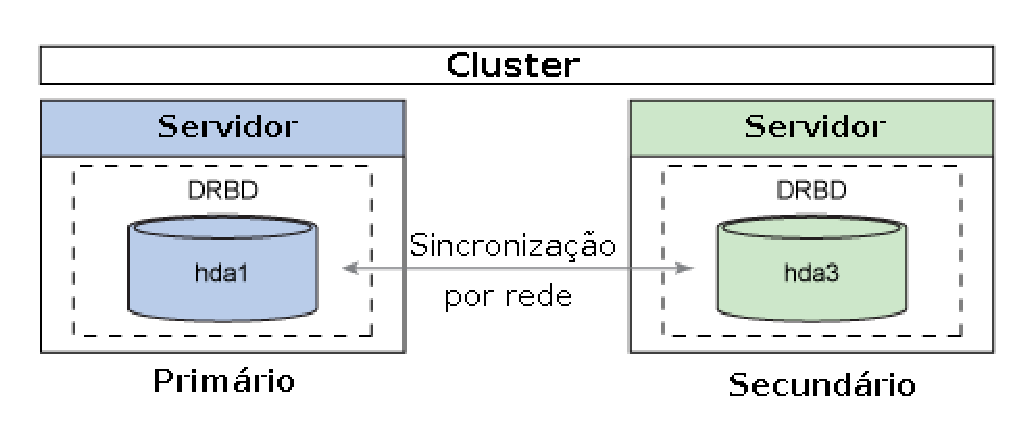
\includegraphics[width=300px]{img/drbd_basic.eps}
 }
 \caption{Exemplo do modelo \textit{master-slave} do \ac{DRBD}.}
 Fonte: \citet{jones2010}
 \label{fig:drbd_basic}
\end{figure}

O \ac{DRBD} pode ser configurado dos seguintes modos \cite{drbd}:
\begin{itemize}
 \item \textit{Single-primary}: ou \textit{master-slave}, neste modo apenas um nó do \textit{cluster} pode ser o nó primário. Neste caso, somente
 o nó primário terá permissão para acessar o dispositivo, ou seja, somente ele poderá fazer operações de leitura e escrita. Já o nó 
 secundário terá apenas uma réplica dos dados;
 \item \textit{Dual-primary}: ou \textit{dual-master}, neste modo existem dois nós primários, nos quais podem ser realizadas operações de leitura e 
 escrita de forma simultânea. Porém, este modo necessita de um sistema de arquivos compartilhados, sendo que neste caso podem ser utilizados os 
 sistemas de arquivos: o \ac{GFS} \cite{gfs} e o \ac{OCFS2} \cite{ocfs2}.
\end{itemize}

\subsubsection{GlusterFS}
\label{section:glusterfs}
O \textit{GlusterFS} \cite{glusterfs} é um sistema de arquivos distribuídos mantido pela \textit{Gluster community}. Esse \textit{software} 
utiliza estrutura de \textit{cluster} e seu principal objetivo é a escalabilidade, ou seja, este possui funcionalidades que facilitam o aumento
da capacidade do \textit{cluster} a partir da inclusão de novos nós.

Na Figura \ref{fig:glusterfs} tem-se dois nós, onde cada nó possui dois discos rígidos, que são denominados \textit{bricks}. 
A partir dos \textit{bricks} o \textit{GlusterFS} constrói um volume lógico que é disponibilizado através da rede para os clientes 
\textit{GlusterFS}. A organização destes \textit{bricks} vai depender do objetivo da aplicação, sendo que uma das formas é a replicação. Esses 
diferentes tipos de configurações serão detalhados a seguir.

\begin{figure}[h!]
 \centering
 \fcolorbox{black}{white}{
  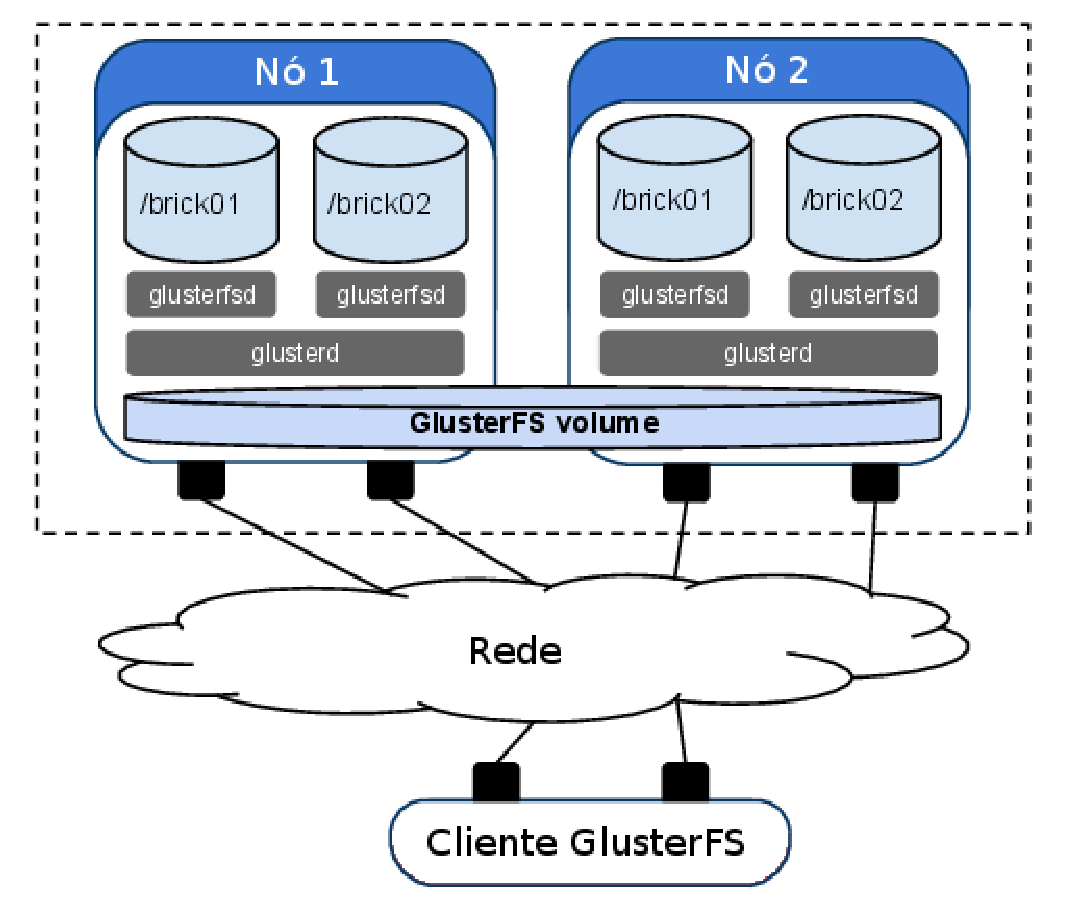
\includegraphics[width=280px]{img/glusterfs.eps}
 }
 \caption{Modelo do \textit{GlusterFS}.}
 Fonte: \citet{davies2013}
 \label{fig:glusterfs}
\end{figure}

O \textit{GlusterFS} suporta diferentes tipos de configurações de volumes, com as opções de distribuição e replicação de dados \cite{glusterfs}:
\begin{itemize}
 \item Volume distribuído: neste tipo os arquivos são distribuídos entre os diferentes \textit{bricks} dos nós. O objetivo deste tipo de 
 configuração é ampliar a capacidade de armazenamento. Desta forma, não tem-se preocupação com a redundância de dados, sendo que no caso de uma
 falha em um nó haverá uma perda de todos dados;
 \item Volume replicado: neste tipo os arquivos são replicados entre os \textit{bricks}, deste modo, tem-se uma redundância, ou seja, caso ocorra
 uma falha em um \textit{brick} não haverá perda de dados;
 \item Volume distribuído e replicado: este é a combinação dos dois tipos de volumes anteriores. Neste caso, é feita a distribuição 
 e a replicação dos arquivos entre os nós;
 \item Volume listrado: neste tipo ocorre a distribuição de um mesmo arquivo entre os \textit{bricks}, ou seja, um arquivo é dividido entre os
 \textit{brick}. Esse tipo é normalmente utilizado para armazenamento de arquivos muito grandes;
 \item Volume distribuído e listrado: este tipo de volume é a combinação do distribuído e do listrado. Neste modo é feita a divisão do arquivo 
 entre \textit{bricks} distintos, sendo que estes são replicados.
\end{itemize}

\subsubsection{Rsync}
\label{section:rsync}
O \textit{Rsync} \cite{rsync} é um \textit{software} desenvolvido e mantido por \textit{Wayne Davison}. Esse \textit{software} prove uma rápida
transferência de arquivos, ou seja, ele faz o sincronismo de arquivos em servidores transferindo dados de um servidor de origem para um de destino.
A Figura \ref{fig:rsync} demonstra o funcionamento do \textit{Rsync}. Observa-se que no \textit{Rsync} tem-se a replicação dos arquivos que
ainda não foram atualizados ou que não existem no servidor de destino. Além disso, o \textit{Rsync} permite uma replicação completa. Neste caso,
tem-se uma replicação onde os arquivos já existentes são sobrescritos.

\begin{figure}[h!]
 \centering
 \fcolorbox{black}{white}{
  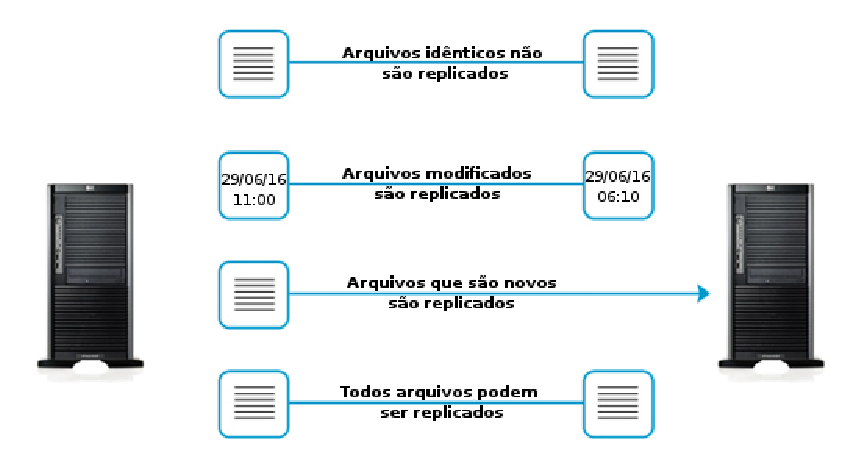
\includegraphics[width=370px]{img/rsync.eps}
 }
 \caption{Transferência de arquivos através do \textit{Rsync}.}
 Fonte: \citet{lopez2012}
 \label{fig:rsync}
\end{figure}

%Algoritmo \cite{tridgell98}

O \textit{Rsync} pode ser configurado como servidor, o que permite que vários clientes possam sincronizar os dados com ele. 
Além disso, o sincronismo pode ser de cliente para cliente, utilizando como transporte o protocolo \ac{SSH} ou através de \textit{sockets}.
Destaca-se que o \textit{Rsync} não faz um sincronismo em tempo real, ou seja, ele faz o sincronismo a partir de uma ação (execução de um comando).

% Ceph RBD
% Swift open stack
% https://wiki.freebsd.org/HAST

\subsubsection{Resumo e software de replicação adotado}
\label{section:replicacaoescolhido}

Na Tabela \ref{tab:replicacao} tem-se uma comparação entre as ferramentas citadas anteriormente. 
A ferramenta adotada para replicação de dados foi o \ac{DRBD}, pois permite a configuração \textit{dual-primary} e também \textit{master-slave}, 
além de suportar a replicação de máquinas virtuais e fazer replicação a nível de bloco. Além disso, essa ferramenta permite a ressincronização 
dos dados de forma automática em caso de um falha \cite{drbd}.

\begin{table}[h!]
\caption{Comparação ferramentas de replicação de dados.}
\label{tab:replicacao}
\begin{center}
\begin{tabular}{|l|p{3.5cm}|p{3.5cm}|p{2cm}|}\hline
\textbf{Características} & \textbf{DRBD} & \textbf{GlusterFS} & \textbf{Rsync} \\\hline
Integração com virtualização & Sim & Sim & Não \\\hline
Dual-primary & Sim & Sim & Não \\\hline
Replicação em tempo real & Sim & Sim & Não \\\hline
Nível de replicação & Bloco & Arquivo & Arquivo \\\hline
Número máximo de nós & 16 & 64 & Ilimitado \\\hline
Distribuições Linux & Suse, Debian, CentOS, Red Hat, Ubuntu & Debian, CentOS, Red Hat, Fedora, Ubuntu & Todas \\\hline
\end{tabular}
\end{center}
\end{table}

O \textit{GlusterFS} poderia ser utilizado, porém este faz uma replicação a nível de arquivo, sendo assim, não é adequada para uma 
solução de alta disponibilidade que utiliza-se de virtualização. 
E, por fim, o \textit{Rsync} não pode ser utilizado pois não executa uma replicação em tempo real, além de não ter sido desenvolvido para
executar em conjunto com a virtualização.

%Pode-se perceber que o \textit{Ceph RBD} não possui a opção de
%\textit{master-slave}. Esse \textit{software} necessita de um \textit{hardware} adicional para sua administração. 

%https://www.reddit.com/r/linux/comments/1qwarp/drbd_vs_glusterfs/
% glusterfs mais escalavel, simples de administrar
% drbd melhor eficiencia(acredito) nivel de bloco, confiavel(10 anos develop)

% drbd: 2 nodes na versão 8 e 16 nodes por stacking / 16 nodes na versão 9

% drbd dispositivo primário e secundário zaminhani2008
% Segundo (ELLENBERG, 2007), a partir da versão 8 do DRBD é possível que,
%dependendo da aplicação, a execução ocorra em todos os nós do cluster
%simultaneamente (Ativo/Ativo). Para tornar isso possível é necessária a
%utilização de um sistema de arquivos exclusivo para cluster, como o OCFS2 6 e o
%GFS 7 por exemplo. Como a abordagem deste trabalho é cluster de alta
%disponibilidade, a utilização do DRBD no modo Ativo/Ativo não será discutida.

% glusterfs https://raobharata.wordpress.com/2012/10/29/qemu-glusterfs-native-integration/
% melhor performace com disco utilizando protocolo gluster file=gluster://path/to

% ceph http://docs.ceph.com/docs/master/start/intro/
% necessita minimo 3 monitores com osd, outra para administração
% precisa openstack + nova
% http://www.server-world.info/en/note?os=Ubuntu_14.04&p=ceph
% https://elkano.org/blog/live-migration-openstack-ubuntu-14-04/

\subsection{Softwares para o gerenciamento de cluster}
\label{section:toolcluster}

Para ser possível implementar uma solução de alta disponibilidade é necessário organizar os servidores em uma estrutura de \textit{cluster},
sendo assim, é interessante a utilização de \textit{softwares} que facilitam o gerenciamento deste \textit{cluster}. Esses \textit{softwares} 
permitem detectar falhas em um nó, sendo elas de \textit{hardware} ou de serviços. Essas ferramentas são conhecidas como \ac{CRM}. 

Após a detecção de uma falha, os \textit{softwares} de gerenciamento de \textit{cluster} executam operações de \textit{failover} e 
\textit{failback}. O \textit{failover} é um processo no qual um servidor recebe os serviços que estavam executando no servidor que falhou. 
Já no \textit{failback} tem-se o retorno dos serviços para o servidor de origem quando este estiver disponível. Esse processo ocorre após o 
\textit{failover} sendo que ele é opcional \cite{bassan2008}. Nas próximas seções tem-se uma breve descrição dos \textit{softwares} de 
gerenciamento de \textit{cluster} que foram estudados.

% \subsubsection{Ceph}
% \label{section:ceph}
% O \textit{Ceph} \cite{ceph} é uma ferramenta com foco no armazenamento de dados distribuídos. Esta ferramenta tem foco em \textit{cluster} 
% de armazenamento, sendo assim ela necessita de outra ferramenta para gerenciar as máquinas virtuais, como por exemplo \textit{OpenStack} 
% \cite{openstack}. Sua arquitetura é composta por um nó administrador, onde tem-se a gerência do \textit{cluster}, e no mínimo dois 
% nós, sendo um para o armazenamento (\textit{Ceph OSD}) e um para o monitoramento (\textit{Ceph Monitor}) e o processamento (\textit{Ceph MDS}) \cite{ceph}.

\subsubsection{Ganeti}
\label{section:ganeti}
O \textit{Ganeti} \cite{ganeti} é um \textit{software} desenvolvido pelo \textit{Google}. Esse \textit{software} é um gerenciador de 
\textit{cluster} de virtualização. Ele foi desenvolvido especificamente para ambientes de virtualização e suporta os hipervisores 
\ac{KVM} \cite{kvm} e \textit{Xen} \cite{xen}. 

Na Figura \ref{fig:ganeti_arquitetura} tem-se a arquitetura do \textit{Ganeti}. O \textit{cluster} é composto por um nó \textit{master}, que 
armazena as configurações e gerencia o \textit{cluster}, e um nó \textit{master candidate}, para o caso do nó \textit{master} falhar. 
Além disso, ele permite a criação de vários nós \textit{slaves}. Destaca-se que todos os nós são responsáveis por prover o ambiente de 
virtualização e armazenar os dados das \acp{VM}, sendo que cada nó pode possuir uma ou mais instâncias de \acp{VM}. Em cada instância 
configura-se dois nós: o nó primário, que a instância executará inicialmente; e o nó secundário, que será utilizado no caso do nó primário falhar.
Além disso, as instâncias também podem ser migradas de um nó para outro de forma manual. 

\begin{figure}[h!]
 \centering
 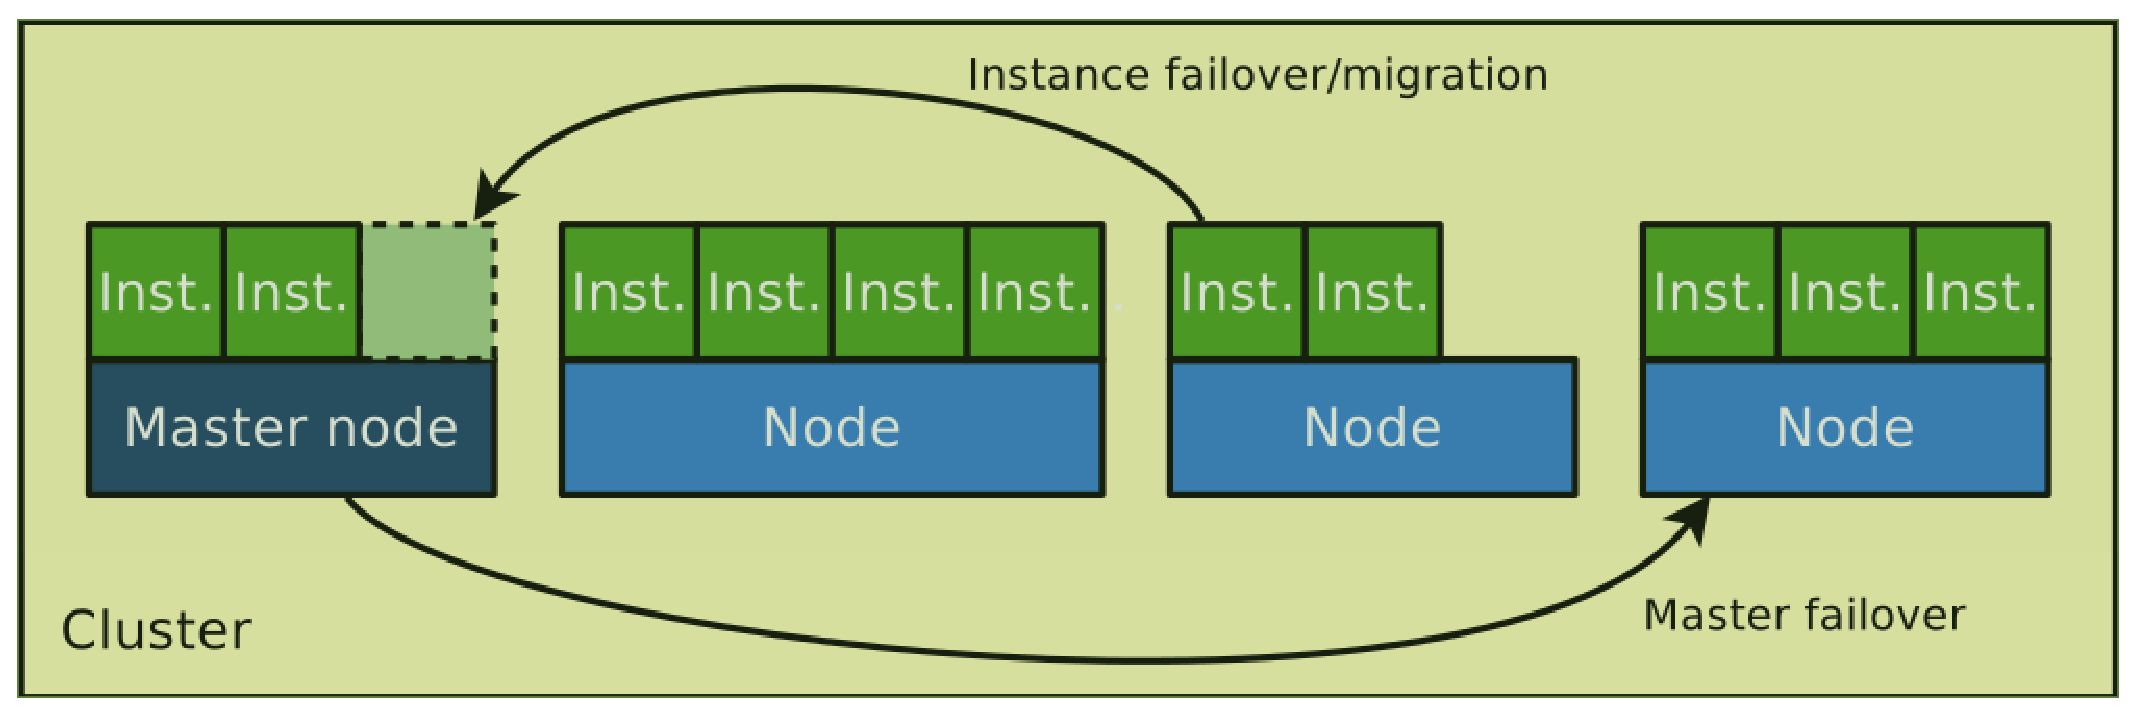
\includegraphics[width=380px]{img/ganeti_arquitetura.eps}
 \caption{Arquitetura do \textit{Ganeti}.}
 Fonte: \citet{carvalho2011}
 \label{fig:ganeti_arquitetura}
\end{figure}

\newpage
As principais funcionalidades do \textit{Ganeti} são \cite{ganeti}:
\begin{itemize}
 \item Criação de instâncias;
 \item Gerenciamento do armazenamento das instâncias;
 \item Iniciar e finalizar instâncias, além de efetuar a migração entre os nós.
\end{itemize}

% ganeti pode ser usado com ceph rdb (RADOS Cluster), ou drbd, ou gluster

\subsubsection{Heartbeat}
\label{section:heartbeat}
O \textit{Heartbeat} é um subprojeto do \textit{Linux-HA} \cite{linuxha}, que desenvolve soluções de alta disponibilidade.
Esse subprojeto é uma aplicação que envia pacotes \textit{keepalive \ac{UDP}}, através da rede, para outras aplicações \textit{Heartbeat}. 
Esses pacotes possuem como objetivo verificar se uma aplicação está ativa.
Destaca-se que esse \textit{software} pode ser utilizado para alta disponibilidade em ambientes de virtualização \cite{reis2009}.

Na Figura \ref{fig:heartbeat} tem-se o \textit{Heartbeat} executando em dois servidores sobre as interfaces de rede dedicadas (\textit{ethX}).
Neste caso, se o nó secundário deixar de receber os sinais do nó primário, este irá tornar-se o nó primário, e iniciará o processo de 
\textit{failover}. 
%com isso, ele receberá o \ac{IP} virtual (\textit{192.168.50.3}) e iniciará os serviços previamente configurados.
\begin{figure}[h!]
 \centering
 \fcolorbox{black}{white}{
  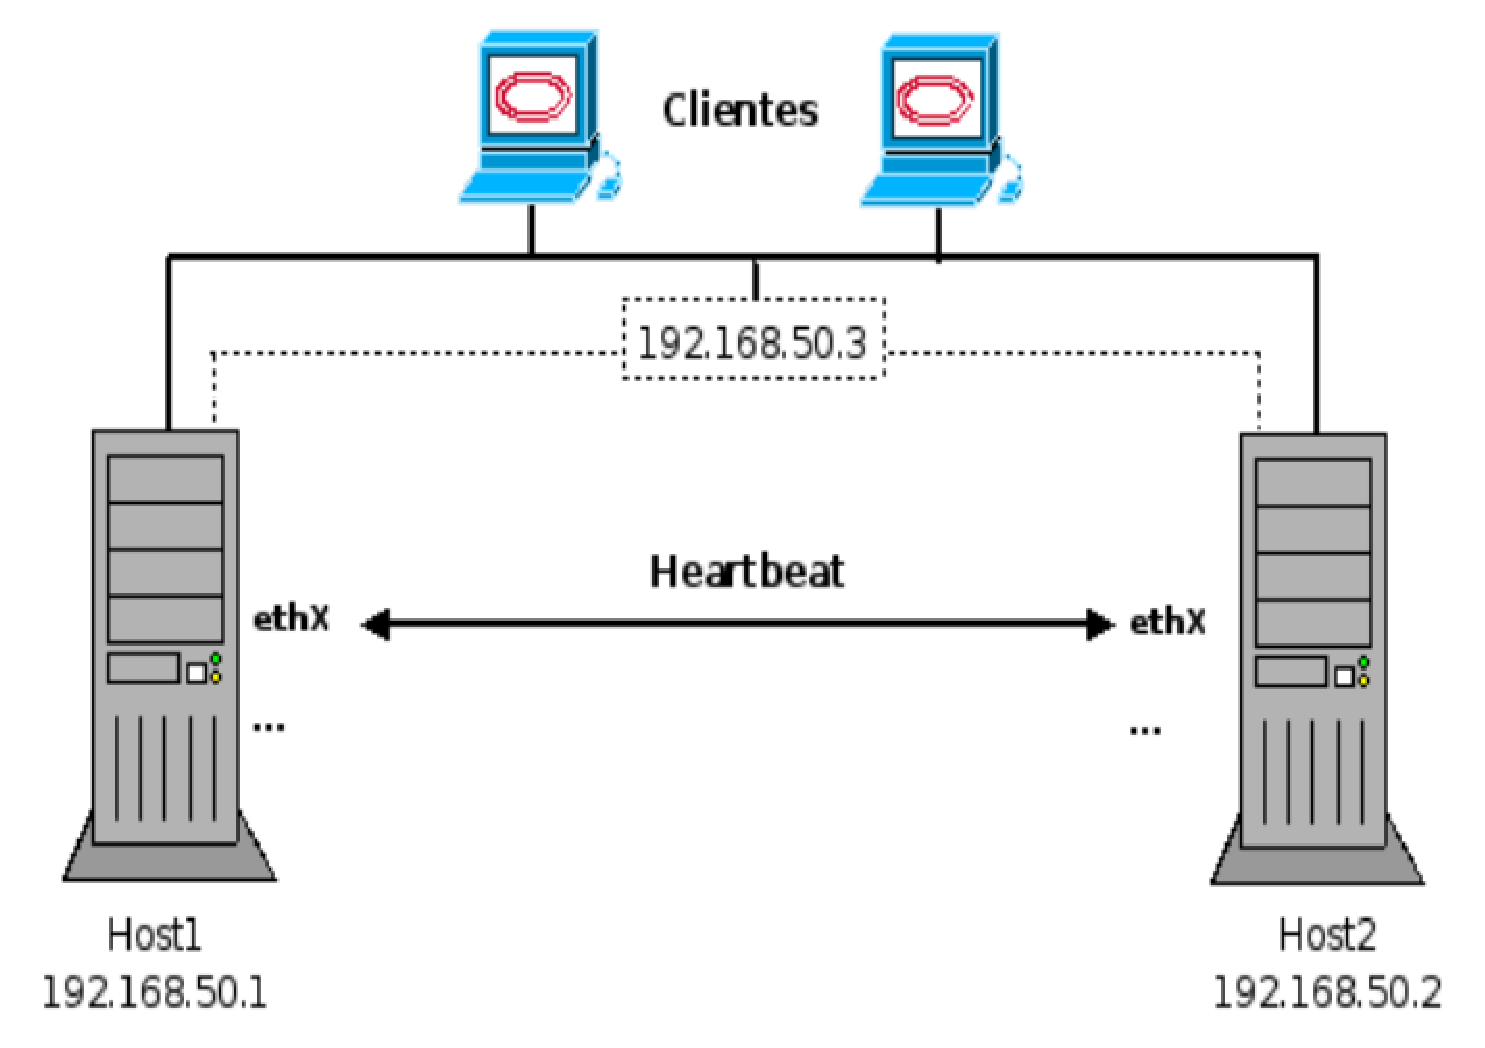
\includegraphics[width=300px]{img/heartbeat.eps}
 }
 \caption{Arquitetura do \textit{Heartbeat}.}
 Fonte: \citet{zaminhani2008}
 \label{fig:heartbeat}
\end{figure}

As principais funcionalidades do \textit{Heartbeat} são \cite{clusterlabs}:
\begin{itemize}
 \item Enviar mensagens entre os nós para a detecção de falhas;
 \item Efetuar os processos de \textit{failover} e \textit{failback};
 \item Iniciar e finalizar serviços nos nós;
\end{itemize}

%exemplo de implementacao heartbeat com virtualizacao = \cite{reis2009}

\subsubsection{Pacemaker}
\label{section:pacemaker}
O \textit{Pacemaker} \cite{pacemaker} é um projeto de código aberto mantido pela \textit{ClusterLabs}, e teve origem com a necessidade de 
aperfeiçoar o \textit{Heartbeat} \cite{heartbeat}. 
O \textit{Pacemaker} pode ser definido como uma ferramenta de recuperação de falhas a nível de serviço \cite{perkov2011}. 

Esse \textit{software} é utilizado juntamente com ferramentas que fazem registro dos nós e troca de mensagens entre os nós do \textit{cluster}.
As ferramentas que podem ser integradas com o \textit{Pacemaker} são \cite{pacemaker}:
\begin{itemize}
 \item \textit{Corosync} \cite{corosync}: é responsável pelo processo de registro dos nós e pelo processo de \textit{failover}.
 %bloqueios distribuídos (utilizados para implementar \ac{LVM} \cite{lvm}, \ac{GFS}, e \ac{OCFS2}). 
 Essa ferramenta derivou do projeto \textit{OpenAIS};
 \item \textit{Heartbeat}: essa ferramenta faz envio de mensagens entre os nós do \textit{cluster}, além de iniciar e finalizar serviços.
\end{itemize}
% outras ferramentas cMAN e Apache Qpid

%Modelos Active/Passive, N+1, N TO N, Split Site ??

Na Figura \ref{fig:pacemaker_tools} tem-se a arquitetura do \textit{Pacemaker}. Como pode ser observado na camada inferior tem-se os nós do 
\textit{cluster}. Na camada superior tem-se o \textit{software} de envio de mensagens e acima deste tem-se o \textit{Pacemaker}. 
Por fim, tem-se os serviços.

\begin{figure}[h!]
 \centering
 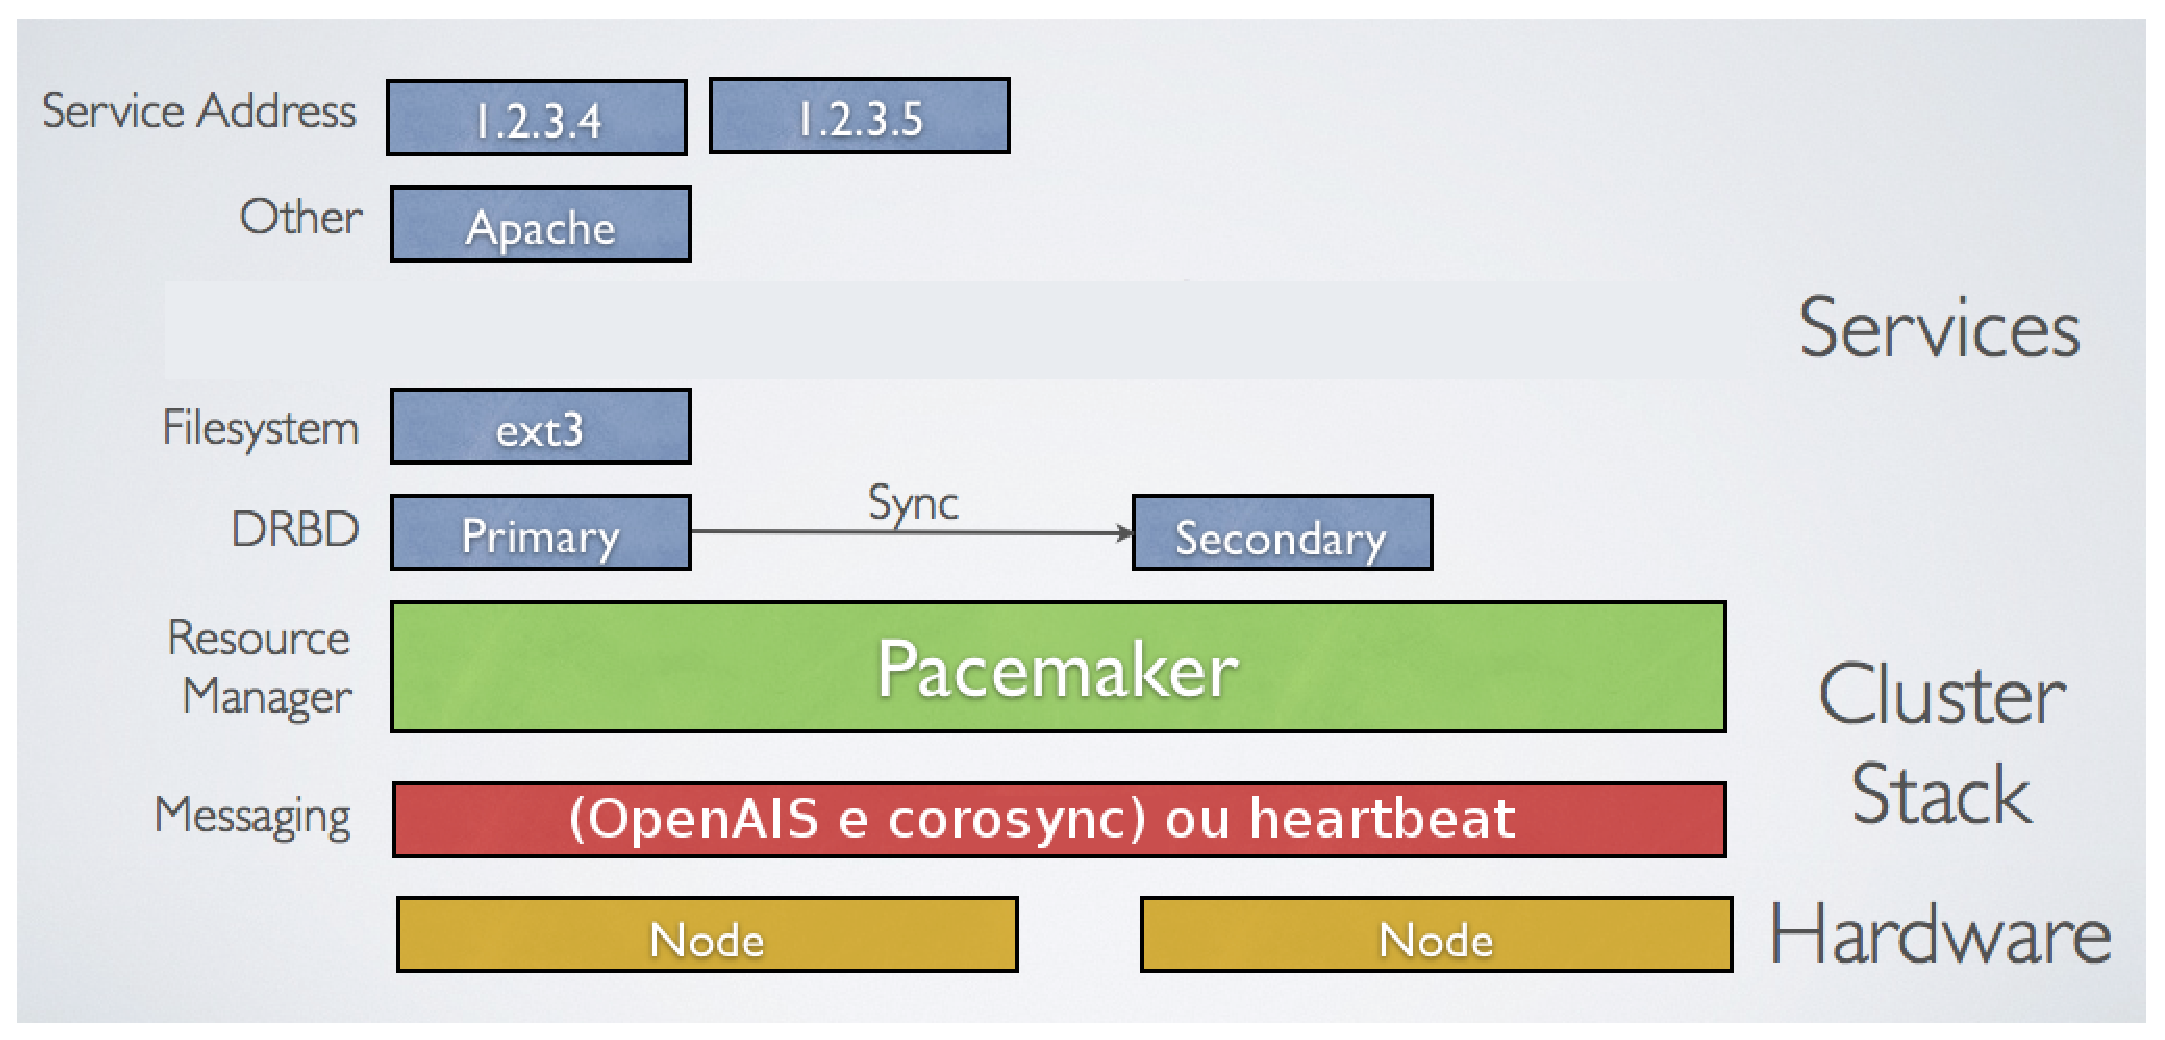
\includegraphics[width=350px]{img/pacemaker_tools.eps}
 \caption{Exemplo da arquitetura do \textit{Pacemaker}.}
 Fonte: \citet{pacemaker}
 \label{fig:pacemaker_tools}
\end{figure}

Entre as principais funcionalidades do \textit{Pacemaker} tem-se:
\begin{itemize}
 \item Iniciar e finalizar os serviços dos nós do \textit{cluster}. Esses serviços podem ser desde um servidor \textit{web} ou uma interface de 
 rede até uma máquina virtual;
 \item Replicação de configuração do \textit{cluster} para todos os nós de forma transparente. Desta forma, a configuração do \textit{cluster} 
 pode ser alterada em qualquer nó;
 \item Eleição de um nó como primário. No caso de uma falha neste nó, um outro será eleito primário.
\end{itemize}

No \textit{Pacemaker} os serviços são denominados recursos (\textit{resources}), esses recursos são monitorados, iniciados e parados.
Também pode-se criar dependências e ordem entre esses recursos, por exemplo, para iniciar um serviço \textit{web} é necessário iniciar 
um \ac{IP} antes. Além disso, existem agentes que são responsáveis pela integração com os diversos serviços e ferramentas. 
Também pode configurá-lo para fazer o \textit{failover}, desta forma caso ocorra uma falha em um nó, o \textit{Pacemaker} fará a inicialização 
dos serviços em outro nó que foi previamente configurado. Essa ferramenta também servirá para recuperar um recurso que falhou, por exemplo, se 
o serviço de banco de dados parar por uma falha qualquer, ele será iniciado novamente.

% Corosync provides pacemaker:
% a mechanism to reliably send messages between nodes,
% notifications when machines appear and disappear
% a list of machines that are up that is consistent throughout the cluster 
% Heartbeat provides:
% a mechanism to reliably send messages between nodes,
% notifications when machines appear and disappear
% a list of machines that are up that is consistent throughout the cluster 
% --
% http://serverfault.com/questions/269831/relation-between-heartbeat-openais-corosync
% well i reached answer on myself! clustering include two part:
% 1.cluster resource management
% 2.infrastructure with massaging layer
% legacy heartbeat is broken into heartbeat message layer and pacemaker so pacemaker is CRM.
% and we have two option on message layer:heartbeat,openais. openais/corosync is preferred as: http://comments.gmane.org/gmane.linux.
%highavailability.user/32355
% There are, however, features in Pacemaker that require OpenAIS which will work only with Corosync, not Heartbeat. Those features are concerned 
% with the distributed lock managers used by cLVM (but not regular LVM), GFS/GFS2, and OCFS2. If you need that functionality, you must select 
% OpenAIS/Corosync. If you do not, you're free to choose.
% as: http://www.clusterlabs.org/wiki/FAQ
% Originally Corosync and OpenAIS were the same thing. Then they split into two parts... the core messaging and membership capabilities are now 
% called Corosync, and OpenAIS retained the layer containing the implementation of the AIS standard.
% Pacemaker itself only needs the Corosync piece in order to function, however some of the applications it can manage (such as OCFS2 and GFS2) 
% require the OpenAIS layer as well.
% so i went to openais/corosync and integrate it with pacemaker.
% --
% There are, however, features in Pacemaker that require OpenAIS which
% will work only with Corosync, not Heartbeat. Those features are
% concerned with the distributed lock managers used by cLVM (but not
% regular LVM), GFS/GFS2, and OCFS2. If you need that functionality, you
% must select OpenAIS/Corosync.
% 
% Pacemaker itself only needs the Corosync piece in order to function, however some of the applications it can manage 
% (such as OCFS2 and GFS2) require the OpenAIS layer as well. 

\subsubsection{Resumo e software de gerenciamento adotado}
\label{section:gerenciadorescolhido}

Na Tabela \ref{tab:clusterger} tem-se uma comparação dos \textit{softwares} de gerenciamento de \textit{cluster}. 
O \textit{software} adotado para gerenciar o ambiente será o \textit{Pacemaker}, pois este possui todos os requisitos para a criação de um 
\textit{cluster} de alta disponibilidade utilizando virtualização. A principal e fundamental característica é o \textit{failover} automático
dos nós, pode-se perceber na tabela que o \textit{Pacemaker} é o único que suporta isto. Além disso, ele possui suporte a migração em tempo real, 
que pode ser utilizada para manutenções. Esse \textit{software} é o único que possui a característica de sincronismo de configuração entre todos 
os nós. Essa ferramenta é indicada no site do \ac{DRBD} para compor um \textit{cluster} de alta disponibilidade \cite{drbd}.
Destaca-se que já foram realizados testes de migração de máquinas virtuais em tempo real utilizando o \textit{Pacemaker}, e obteve-se 
bons resultados.

\begin{table}[h!]
\caption{Comparação entre ferramentas de gerenciamento de \textit{cluster}.}
\label{tab:clusterger}
\begin{center}
\begin{tabular}{|p{4cm}|p{2cm}|p{3.5cm}|p{3.5cm}|}\hline
\textbf{Características} & \textbf{Ganeti} & \textbf{Heartbeat} & \textbf{Pacemaker} \\\hline
Suporte nativo a virtualização & Sim & Não & Sim \\\hline
Migração de \acp{VM} em tempo real & Sim & Não & Sim \\\hline
Failover e failback automáticos & Não & Não & Sim \\\hline
Sincronismo de configuração entre os nós & Não & Não & Sim \\\hline
Distribuições Linux & Todas & Red Hat, CentOS, Fedora, Suse, Debian, Ubuntu & Red Hat, CentOS, Fedora, Suse, Debian, Ubuntu \\\hline
\end{tabular}
\end{center}
\end{table}

Pode-se perceber que o \textit{software} \textit{Ganeti} não faz o \textit{failover} de forma automática, o que é necessário para esta 
implementação, sendo assim essa ferramenta é normalmente utilizada em ambientes com foco na segurança dos dados, pois os dados podem ser 
facilmente recuperados.
É possível também implementar uma solução de alta disponibilidade com a ferramenta \textit{Heartbeat}. Porém, neste caso seria necessário criar 
um conjunto de \textit{scripts} para a migração das máquinas virtuais.

% Já o \textit{Pacemaker} é o único que possui a característica de sincronismo de configuração entre todos os nós, no entanto, isto não é uma
% característica essencial para o desenvolvimento deste trabalho. Além disso, o \textit{Pacemaker} não possui a opção nativa de migração em tempo
% real das \acp{VM}.

% Pode-se observar que o \textit{software} \textit{Ceph} possui suporte apenas para a detecção e recuperação a nível de nó. De fato, esse 
% \textit{software} tem foco em \textit{cluster} de armazenamento, desta forma necessitando de outra ferramenta para gerenciar a migração de 
% máquinas virtuais. Além disso, essa ferramenta necessita de um \textit{hardware} especifico para administração do \textit{cluster}.

% O \textit{software} escolhido para gerenciar o ambiente que será criado neste trabalho foi a ferramenta de código aberto \textit{Pacemaker}. 
% Esse \textit{software} possui todos os requisitos para criar um \textit{cluster} de alta disponibilidade, sendo que, também pode ser configurada 
% para fazer monitoramento e recuperação tanto a nível de nó quanto a nível de recurso. Além disso, ela possui a característica de sincronismo de 
% configuração entre todos os nós que é exclusiva. Destaca-se que essa ferramenta é indicada no site do \ac{DRBD} para compor um \textit{cluster} 
% de alta disponibilidade \cite{drbd}.


\section{Considerações finais}

Neste capítulo foram apresentados os serviços críticos. Posteriormente foram apresentadas ferramentas para implementação de alta disponibilidade 
e selecionada a mais adequada para o ambiente real da empresa. No próximo capítulo será apresentada a implementação da solução de alta 
disponibilidade, efetuado testes e apresentos os resultados.

